\documentclass[11pt,a4paper,oneside]{book}

% Packages
\usepackage{caption}
  \captionsetup{font=footnotesize}
\usepackage{epigraph}
\usepackage{float}
\usepackage{fullpage}
\usepackage{geometry}
  \geometry{verbose,tmargin=2cm,bmargin=2.5cm,lmargin=2.5cm,rmargin=2.5cm,footskip=1.5cm}
\usepackage{graphicx}
\usepackage[colorlinks=true, linkcolor=blue, citecolor=blue]{hyperref}
\usepackage{mathtools}
\usepackage[round]{natbib}
  \bibliographystyle{plainnat}
\usepackage{setspace}
  \onehalfspacing
\usepackage[textsize=scriptsize]{todonotes}

% User-defined commands
\newcommand{\latex}{\LaTeX{}} % latex symbol

% Path for graphs
\graphicspath{{images/}}


% ===== TITLE =====================================================================================
\title{From Crosses to Micro Foundations:\\
The Stepping Stone from Monetary Economics in the IS-LM Model to the New-Keynesian paradigm}

\author{
  (coordinator)
  \and
  Roxane Achteri
  \and
  Fabio Bernasconi
  \and
  Graant Boraas
  \and
  Gabriel Buchli
  \and
  Fabiola Cappiello Segura
  \and
  Antonin Carratero
  \and
  Rui Cui
  \and
  Juana De Rosa
  \and
  Oliver Dislich
  \and
  Alexandru Dolea
  \and
  Maximilian Eid
  \and
  Sofia Grimoldi
  \and
  Julian Haussmann
  \and
  Julien Iff
  \and
  Stephanie Jordan
  \and
  Luc-Vincent Lauper
  \and
  Leo Leibundgut
  \and
  Calvin Limat
  \and
  Elio Magnani
  \and
  Matteo Monga
  \and
  Maximilian M\"{o}stl
  \and
  Samuel Scuotto
  \and
  Eva Pampurik
  \and
  Michel Voutat
  \and
  Daniela Wendler
  \and
  Anton Xu
}
% =================================================================================================

\begin{document}
\frontmatter
\maketitle

% ===== ABOUT THIS NOTES ==========================================================================
\chapter{About these notes}
\epigraph{If you can't explain it simply, you don't understand it well enough.}{\textit{Attributed to} Albert Einstein}

The main objective of these notes is to create a reference document that can be useful to all students who want to review bridge the gap between the IS-LM model and the New Keynesian paradigm.

As a chapter author, your job is \textbf{NOT} to put together a lot of information that is difficult and tiring to read. Keep always in mind that measuring the quality of your chapter by the lines or pages written is like measuring aircraft building progress by weight.\footnote{This is an adaptation of a code from Bill Gates that says "Measuring programming progress by lines of code is like measuring aircraft building progress by weight".} Your job is to facilitate learning and understanding. To explain something to somebody else requires that you deeply \textbf{understand} what you are explaining. Hence, your first job is to understand the concepts you need to explain. Then you need to reflect in which is the best way to present those concepts to facilitate learning. Lastly, you have to make sure that the document produced actually accomplishes the purpose for which it is created.

The main sources of information you have are the class slides and what is discussed during the lectures. However, your chapter should not be a transcript of what was explained during each session. You need to create a narrative that connects the concepts covered and helps the reader understand these concepts and the context in which they are relevant. Look into the textbooks, recommended readings, references, etc. and enhance the information covered in the class.

This work is licensed under a \href{http://creativecommons.org/licenses/by-nc/4.0/}{Creative Commons Attribution-NonCommercial 4.0 International License}.

\newpage
\section*{FAQs}
\subsection*{How long should the chapter be?}
As short as possible. Your objective is that every time you explain something you explain it with as few words/sentences as possible, provided you give a great explanation. The evaluation is on the quality of what you produce. There is no quantity/quality trade-off. If you cover many concepts/facts poorly, you will get a poor grade. If you cover a few topics greatly, you will get a good grade. If you cover many topics greatly, you will get a great grade.

\subsection*{Can external sources be used?}
You \textbf{should} use external sources. Do not copy/paste. Understand and digest every new piece of information before you add it to your chapter. Cite properly, see Section \ref{sec:citations}.

There is lots of information out there related to the topics you want to cover in your chapter. It is humanly impossible to review \textit{all} that information in order to write anything. Try to focus on academic/policy work. That is, give priority to academic articles in scientific journals or journals of central banks, working papers, books, and policy reports. There are exceptions but newspaper's articles and op-eds tend to either contain unimportant information or rephrase ideas and arguments lay out in academic outlets.

Not all academic work is equally valuable for your review. The rank of the journal and the number of citations of an article are positively correlated with its importance but this relationship is far from being a one-to-one matter. There is no way around of reading the article and assessing the value of the ideas/arguments in it. Never use authority as an argument. It is not the case that because the author of an statement has a Nobel prize or is a well-known academic that the statement becomes true or valuable.

\subsection*{Should the content be theoretical or empirical?}
Both. You want to present ideas and you want to contrast these ideas with evidence. That is what Science is about. And Science is what we use to create knowledge. And your chapter will be a great summary of all human knowledge on the topic(s) you are working on. Of course, depending on the topic(s) covered by your chapter the balance between theory and evidence needs to be different. You want to balance two with the objective to maximise how understandable and clear your chapter is.\footnote{Your Professor knows the evidence, do not try to earn points by signalling you have read a lot. Show that you have understood so well what you have read that you can explain it very well.}

\subsection*{Should the chapter follow a specific organization scheme?}
No. Should it be organised to maximise how understandable it is? Definitely. In this regard, to have an introduction tends to be helpful. The purpose of the introduction is to provide motivation and to lay out the topics covered in the chapter.



\newpage
\tableofcontents
\listoffigures
\listoftables
% =================================================================================================

\mainmatter

% ===== TEMPLATE CHAPTER ==========================================================================
\chapter{Template chapter}
\label{ch:template_chapter}
In this chapter you can find a short guideline on how to properly design your chapter. The information here should be almost enough to write your chapter. You should only need external sources to clarify questions you might have. In other words, \textbf{try to keep your document as simple as possible}.

Please use British English.

The best online reference for \latex is the \href{https://en.wikibooks.org/wiki/LaTeX}{Wikibook on \latex}. Moreover, a Google search tends to solve more of the problems one might face.

% ----- DOCUMENT STRUCTURE ------------------------------------------------------------------------
\section{This is a section}
\label{sec:document_structure}
Organising the information you want to present on your chapter is as important as the information itself. When your write your chapter, you can use sections, subsections, and even \textit{subsubsections}. Make sure not to over do it.

For more information on document structure see \href{https://en.wikibooks.org/wiki/LaTeX/Document_Structure}{this} section the \latex Wikibook.
\section{This is another section}
\subsection{This is a subsection}
\subsubsection{And this is a subsubsection}
% -------------------------------------------------------------------------------------------------

% ----- FLOATS ------------------------------------------------------------------------------------
\section{How to present a graph or table}
\label{sec:floats}
To use a graphs we need to create a float-figure like this one:
% ----- BEGIN GRAPH
\begin{figure}[h!]
  \centering
    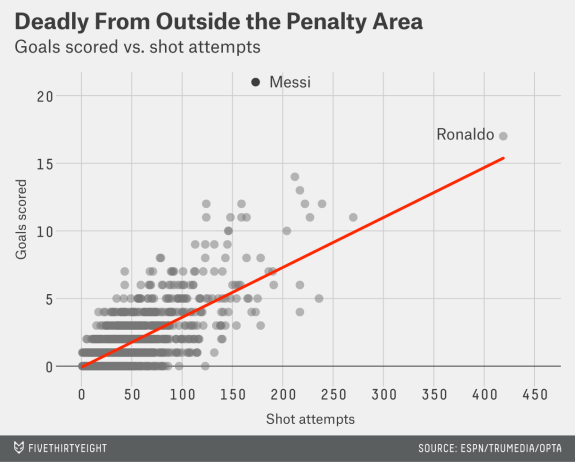
\includegraphics[width=0.25\textwidth]{example}
    \caption{The capiton of each graph should contain a brief description of what appears in the graphs (if the table in the graph is not enough), all the relevant information regarding the type of data displayed, its source, and (if need it) the author of the graph.}
    \label{fig:messi_vs_ronaldo}
\end{figure}
% ----- END GRAPH

Note that all files that contain graphs are saved in the folder \textit{images}. The preferred format for a graph is EPS.

A Table can be created easily by:
% ----- BEGIN TABLE
\begin{table}[h!]
  \centering
    \begin{tabular}{| l c r |}
    \hline
    1 & 2 & 3 \\
    4 & 5 & 6 \\
    7 & 8 & 9 \\
    \hline
    \end{tabular}
  \caption{A simple table.}
  \label{tab:simple_table}
\end{table}
% ----- END TABLE

Creating rich tables can be cumbersome. There are online tools that can help, like \href{https://www.tablesgenerator.com/}{tablesgenerator.com}.

For more information on floats see \href{https://en.wikibooks.org/wiki/LaTeX/Floats,_Figures_and_Captions}{this} section the \latex Wikibook.
% -------------------------------------------------------------------------------------------------

% ----- CITATION ----------------------------------------------------------------------------------
\section{How to cite books, articles, and other parts of the same document}
\label{sec:citations}
The management of a bibliography in \latex is extremely important. If properly done, it can save lots of time and effort. The bibliography in this document is organised as follows. There is a file, named "monetary.bib" in that contains all the information on the items cited. Strictly speaking this file is a BiBTeX file. In order to cite an item, the first thing you need to do is to add that item to the BibTeX file. To do so, you can either use a bibliography manager, such as \href{http://www.jabref.org/}{JabRef} or you can directly edit the BiBTeX file. I strongly recommend you use the first option if you are new to \latex.

Then you need to cite the item within the document. Here you have a citation of an academic article: \citet*{Cooley_Hansen_1989}. Books are cited exactly in the same way within the document: \citet*{Blanchard_2017}. For more information on bibliography management see \href{https://en.wikibooks.org/wiki/LaTeX/Bibliography_Management}{this} section the \latex Wikibook.

To reference another part of the document is very easy, it only requires creating a label and a reference: see section \ref{sec:citations}. You also use cross-references to refer to figures and tables, like Figure \ref{fig:messi_vs_ronaldo} or Table \ref{tab:simple_table}. For more information on labels and cross-referencing see \href{https://en.wikibooks.org/wiki/LaTeX/Labels_and_Cross-referencing}{this} section the \latex Wikibook.
% -------------------------------------------------------------------------------------------------

% ----- MATH --------------------------------------------------------------------------------------
\section{How to present equations}
\label{sec:math}
In \latex it is very easy to work with equations and mathematical expresions. For example one can easily insert mathematical expressions in the text by writting $ a = \frac{b}{c} \times \beta $. Equations can also be inserted by:

% ----- BEGIN EQUATION
\begin{equation}
  f(x)=(x+a)(x+b)
  \label{eq:function}
\end{equation}
% ----- END EQUATION

Equations can also be referenced, like Equation \ref{eq:function}. For more information on mathematics in \latex see \href{https://en.wikibooks.org/wiki/LaTeX/Mathematics}{this} section the \latex Wikibook.
% -------------------------------------------------------------------------------------------------

% =================================================================================================
\part{Overview of Modern Monetary Policy}
% ===== WHAT WE KNOW ==============================================================================
\chapter{What We Know}
\epigraph{Inflation is always and everywhere a monetary phenomenon.}{\citet{Friedman_1963}}

This sentence might not seem all too odd for an student of introductory Macroeconomics, right? When learning about basic Economics, it makes sense as to why changes in the money supply, for instance, can cause inflation. The deeper one goes, however, the less clear this relationship seems. This chapter aims to give a sense of what we know about monetary policy and we will thus return to this quote further on.

In this chapter, we provide a refresher of certain concepts that you should already be familiar with. In Section \ref{sec:monetary_policy_and_monetary_economics}, we familiarize with the concepts of Monetary Policy and Monetary Economics, while also clarifying the tools and goals of Monetary Economics. In Section \ref{sec:consensus}, we give a short overview of the economic consensus about the effects of Monetary Policy. In Sections \ref{sec:quantity_theory}, and \ref{sec:IS_LM}, we lay down two basic theoretical frameworks, the quantity theory of money and the IS-LM model, to discuss their policy implications and how well they are able to account for what we observe in the date. Finally, in Section \ref{sec:money_growth_and_inflation}, we look at the relationship between money growth and inflation and then (\ref{sec:enjoy_with_care}) we try to explain some of the reasons why these models have a hard time explaining the empirical data.

% ----- Monetary Policy and Monetary Economics ----------------------------------------------------
\section{Monetary Policy and Monetary Economics}
\label{sec:monetary_policy_and_monetary_economics}

What is exactly the difference between \textit{Monetary Policy} and \textit{Monetary Economics}? At first sight they seem tightly related, and in a certain way they are. The term \textit{Monetary Policy} is used to describe how a Central Bank manages its tools in order to achieve the policy goals set in its mandate. By “the SNB’s monetary policy” we thus describe how the Swiss National Bank acted within a certain time period. \textit{Monetary Economics}, on the other hand, tries to lay out the mechanisms through which policy tools affect economic outcomes and policy goals. Empirical findings in the domain of monetary economics should be useful to central bankers in the conduct of monetary policy, helping them choose the most appropriate policy tools for the policy goals.\todo[inline]{This difference is important. It can be better explained.}

In order make these definitions less abstract, the terms policy goals and policy tools need to be clarified. Although \textit{policy goals} can significantly differ, many Central Banks aim at keeping inflation low and stable. The Swiss National Bank, the European Central Bank and the Fed all share the goal of keeping the price level stable. However, the Fed also has the goals of maximum employment, … and moderate long-term interest rates.\todo{Visualisation (table?) of stated goals for different central banks across countries.}

Since the central bank has a large set of tools at its disposal, to simplify our analysis, we construct a stylized framework with two main goals and four tools. In Table \ref{tab:policy_goals_tools} we listed a simplified set of tools and goals.

% ----- BEGIN TABLE
\begin{table}[h!]
  \centering
    \begin{tabular}{ p{7cm} | p{7cm} }
	\textbf{Goals} & \textbf{Tools} \\
    \hline
       Low and stable inflation &  Quantity of money\\
	Stabilize output around potential, avoid & Interest rate  \\
	or limit recessions and booms & Quantitative easing \\
	& Macroprudential tools \\
    \end{tabular}
  \caption{Simplified framework of tools and goals for monetary policy}
  \label{tab:policy_goals_tools}
\end{table}
% ----- END TABLE

\todo[inline]{The reason why we simplify needs to be explained. We need a theoretical framework to analyse all countries without getting lost in the details.}

We define two main goals of central banks:
\begin{itemize}
  \item \textbf{Low and stable inflation}, usually defined as an inflation rate in the range of 1-3\% per year and that can still be controlled by the Central Bank. For instance, the FED defines an inflation rate of 2\% per year as in line with the long-term goal of price stability.\todo{Proper citation of FED technical report.}
  \item \textbf{Stabilize output around potential, avoid or limit recessions and booms}. Central Banks should aim at smoothing recessions and booms, without letting output or employment fluctuate too much across business cycles.
\end{itemize}
\todo[inline]{Both goals need further development and justification.}

We define the following policy tools:
\begin{itemize}
  \item \textbf{Quantity of money}: The Central Bank can affect the money supply through open market operations, by participating in the market for bonds or other suitable assets. A central bank that sells its government bonds' holdings, receives an amount of money, which is therefore taken out of the economy. As a result, there is a lower money supply, which has eventually been shrunken by the central bank. The quantity of money can also be affected through reserve requirements. These reserve requirements are being set by the central bank and executed by commercial banks. They are expressed as a percentage of the demand deposits owed to the customers of the bank. A reduction in the reserve ratio increases the amount that banks can loan out, increasing the money multiplier and thus the money supply. A third way for the Central Bank to affect money supply is through the interest rate at which commercial banks can borrow reserves from the Central Bank. Changes in this interest rate can stimulate or discourage borrowing. For instance, a reduction in this interest rate will increase borrowings by commercial banks and increase the money supply.\todo[inline]{A better summary can be constructed gathering information from websites of CBs (learning the details of how it is done).}
  \item \textbf{Interest rate}: Central banks can also target the interest rate and accommodate the demand for money, instead of controlling the supply, in order to achieve the targeted interest rate. In the forecasting models of many central banks the interest rates turned out to be sufficient statistics of monetary policy and are becoming a more popular tool compared to focusing on only money supply. The Fed, for instance, targets the Federal Funds rate, which is a short-term interest rate that commercial banks charge on each other for overnight loans. By deciding to set a lower or higher target, they influence short-term interest rates in the public markets too. Central Banks control more than one interest rate. For instance, the Fed sets the rate it pays on reserves and the rate that commercial banks have to pay on the reserves they borrow from the Fed. The two rates are used to prevent too large fluctuations in the target rate, which is the Federal Funds rate. The ECB also sets the interest rate at which commercial banks can borrow reserves overnight and the interest rate paid to commercial banks on their deposits at the Central Bank and uses both rates to keep the overnight rate on target.\footnote{See \citep*[pp. 411-417]{Mishkin_2016}.}
  \todo{Not clear this reference is needed.}
  \todo[inline]{There is a mix between interest rate targeting as a policy framework and the policy rate as a tool. At this point, we need a short summary of how we got to the assumption that CBs control the interest rate (in reality they don't!).}
  \item \textbf{Unconventional Monetary Policy}: \todo{Here we group all policy instruments that do not typically appear in formal (mathematical) models.}
  \begin{itemize}
    \item \textit{Quantitative easing}: Central Banks can also employ unconventional tools. There are two main rationale for quantitative easing and non-conventional monetary policy: the financial system may be having troubles allocating resources properly, or the short-term nominal interest rate may be near zero where it can't be lowered further due to an adverse shock. The interest rate usually addressed by conventional policies is the money market's. The capital markets, however, determine the long run interest rate and this one is particularly important for firms that need to finance their - mostly long term - investment projects. Therefore, the long run interest rate is crucial for economic growth and investments. Under quantitative easing the central bank resorts to buying riskier securities with longer maturities than usual to drive long term interest rates down. It is thus a special case of open-market operations by the central bank through purchases of long-term government or commercial bonds, in order to flatten the yield curve by lowering long-term interest rates.
    \todo[inline]{What we need at this point is a short summary of what quantitative easing is. Not why it has been implemented, the objectives that may target, nor what its effects might be.}
    \item \textit{Macro-prudential tools:} Generally speaking, macro-prudential tools are used to strengthen the financial system as a whole and thus increase its resilience. Especially after the global financial crisis and since macroeconomic and financial imbalances are often due to an unhealthy international financial system, it was essential to find a financial supervisor that would be able to prevent systematic risk and recognize economic imbalances. The Fed, for instance, in addition to supervising the financial stability of individual institutions, should also take into account risks for the financial system as a whole or for a part of it by exercising its powers to supervise and regulate the banking system.
    \todo[inline]{At this point, we want to define and explain what macro-prudential tools are. Not their effect, importance, nor how they should be used. If one would like to go discuss their effects \citet*{ABG_2018} would be a good starting point.}
  \end{itemize}
\end{itemize}
% -------------------------------------------------------------------------------------------------

% ----- The consensus on Monetary Policy ----------------------------------------------------------
\section{The \textit{consensus} on Monetary Policy in the short and long run}
\label{sec:consensus}
At the beginning of the chapter we introduced the famous quote by Friedman regarding inflation. Today there is still a certain agreement with this definition.\todo{It's not a definition.}

The general consensus among economists is that, in the \textit{long run}, monetary policy only causes hyperinflation\todo{Not correct.}. Monetary policy cannot, over the long run, affect real economic variables and has no effect on the long run employment rate. And since hyperinflation is considered costly for the economy, central bankers need to weigh up costs and benefits carefully, when choosing the long run inflation rate target.

In the \textit{short run}, however, the consensus is that monetary policy can affect real economic variables such as output and employment, in addition to affecting the exchange rate, asset prices and the stock market prices.

\todo[inline]{This is an important section. The aim is to present the framework (the consensus) within which Economics has thought about Monetary Policy. Some remarks are necessary. First, in science, consensus does not imply truth. Second, this consensus is the outcome of several decades of research. Hence, there is both empirical evidence and a body of theoretical work that explain why the consensus is what it is today and not something else. These reasons need to be (briefly) explained. Thirdly, this consensus should be understood as a guideline to make sense of most of the existing research not as a limitation to think about Monetary phenomena.}
% -------------------------------------------------------------------------------------------------

% ----- The most basic Monetary Economics ---------------------------------------------------------
\section{The most basic Monetary Economics}
\label{sec:most_basic_Monetary_Economics}
\todo[inline]{It is a good idea to have a chapter to review the two most basic frameworks used to think about Monetary Economics and Monetary Policy. Namely, the Quantity Theory of Money and the IS-LM Model. It is also a good idea to confront both frameworks with the data and discuss its weaknesses. However, the essential feature of this chapter has to be an effective summary of each framework. Only then, the indispensable and valuable criticism can be added.}

\subsection{The Quantity Theory of Money}
\label{sec:quantity_theory}

The Quantity Theory of money is the foundation of monetarism\todo{What is monetarism?} and tries to explain changes in the general level of commodity prices. The doctrine states that changes in the purchasing power of money are mainly determined by changes in the quantity of the money stock in circulation.
\todo[inline]{Do not mix the debate on schools of thought with purely explaining the theory. Maybe \citet{Humphrey_1974} is not the right reference.}

The quantity theory of money has taken different forms over time, depending on the quantity equation that lied at its basis. For a review of the changes see \citet*{Friedman_1970}.
It is however important to remember that under all different forms, the quantity equation always remains a tautology \citep*[p. 195]{Friedman_1970}.\todo{Requires much more explanation. Not understandable as it stands.}

The quantity equation is then:
% ----- BEGIN EQUATION
\begin{equation}
\label{eq:QTM}
  M \times V = P  \times Y\text{,}
\end{equation}
% ----- END EQUATION
where $M$ is the quantity of money supplied by the central bank, the velocity $V$ is the income velocity of money, $P$ is the price level, and $Y$ the economic output.

To develop the theory, it's important to understand the assumptions behind each variable.

\textbf{The income velocity of money V}, is to interpret as the average number of times the stock of money is used to buy all final goods in the economy. It is defined as the ratio of nominal GDP over the quantity of money. Velocity reflects changes in the demand for money, which is assumed to change slowly, for instance due to changes in technology. A technological improvement that decreases the real money balances held by people in each period would increase velocity. Velocity should thus be constant, at least in the short run.

\textbf{The output Y}, real GDP, is solely determined by the factors of production and the efficiency with which they are combined, and can increase thanks to technological progress. It is assumed that the economy tends to the state of full employment, such that the number of goods and services sold is at its current maximum.

\textbf{The stock of money M}, is decided by the Central Bank and should be easily identifiable. We already discussed in section \ref{subsec:tools} how the Central Bank may affect this variable in practice.

\textbf{The price level P} equals the GDP defalcator and is assumed to be fully flexible in order to keep output in the economy unaffected by monetary policy. The economy needs thus to be perfectly competitive, such that no firm will hold enough market power to be able to manipulate the prices and wages they charge.
\todo[inline]{This \textit{discussion} on the variables of Eqaution \ref{eq:QTM} is not well framed. First, it needs to be clear what is the difference between the \textbf{theoretical concepts} represented in the equation and their \textbf{empirical counterparts}. This is a potentially very interesting aspect to think about. It can be used to explain how difficult can it be to bring to the data seemingly \textit{simple} theories. Second, it is interesting to discuss how has evolved across time the interpretation that economists have given to the Quantitative Theory of Money. However, this cannot be mixed with the first point.}

If the quantity theory is correct in its predictions, the Central Bank cannot mitigate recessions or slow down booms during the business cycle, since output is given by factors that cannot be influenced by the monetary policy of the central bank. Increases or reductions in the growth rate of money supply are absorbed by inflation. It reaches thus different conclusions with respect to today's consensus among economists. Central Banks should only aim at keeping the growth rate of money supply under tight control in order to achieve price stability.\todo{Interesting discussion. To be expanded and improved.}

\subsubsection{The Quantity Theory of Money against the data}
\label{sec:quantity_theory_against_data}
\todo[inline]{It is a good idea to confront the assumptions of the quantity theory of money against the data. However, a good critic needs to understand not only what the theory formally states but also what it \textit{means}.}

Figure \ref{fig:M2_velocity}\todo{Get raw data and plot it using own format. Why seasonally adjust?} shows that the velocity of money has not been constant neither in the short-run nor in the long run.

% ----- BEGIN GRAPH
\begin{figure}[h]
  \centering
    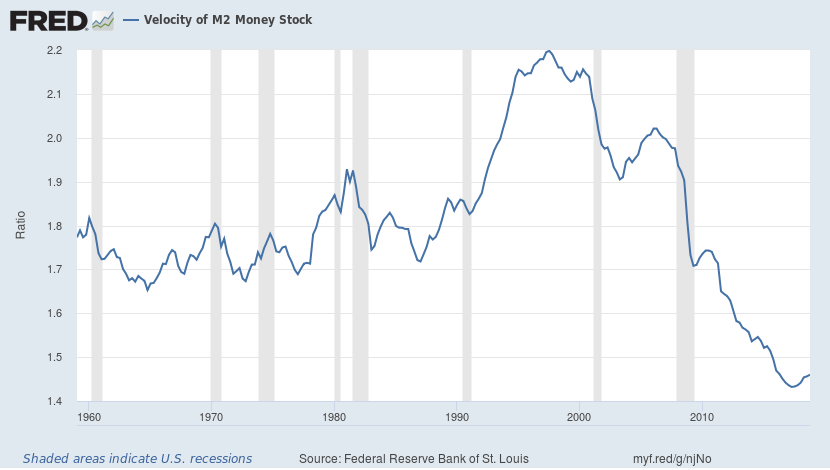
\includegraphics[width=0.6\textwidth]{M2_velocity.png}
    \caption{Velocity of the M2 Money stock, calculated as the ratio of quarterly GDP (series GDP) to the quarterly average of M2 money stock (series M2SL). Quarterly data from 1959 to 2018, seasonally adjusted. Source: Federal Reserve Bank of St. Louis, Velocity of M2 Money Stock [M2V], retrieved from FRED, Federal Reserve Bank of St. Louis; https://fred.stlouisfed.org/series/M2V, March 18, 2019.}
    \label{fig:M2_velocity}
\end{figure}
% ----- END GRAPH

Figure \ref{fig:unempl_US}\todo{Get raw data and plot it using own format. Why seasonally adjust?} shows that the unemployment rate fluctuates a lot and, consequently, $Y$ might not reach full capacity.

% ----- BEGIN GRAPH
\begin{figure}[H]
  \centering
    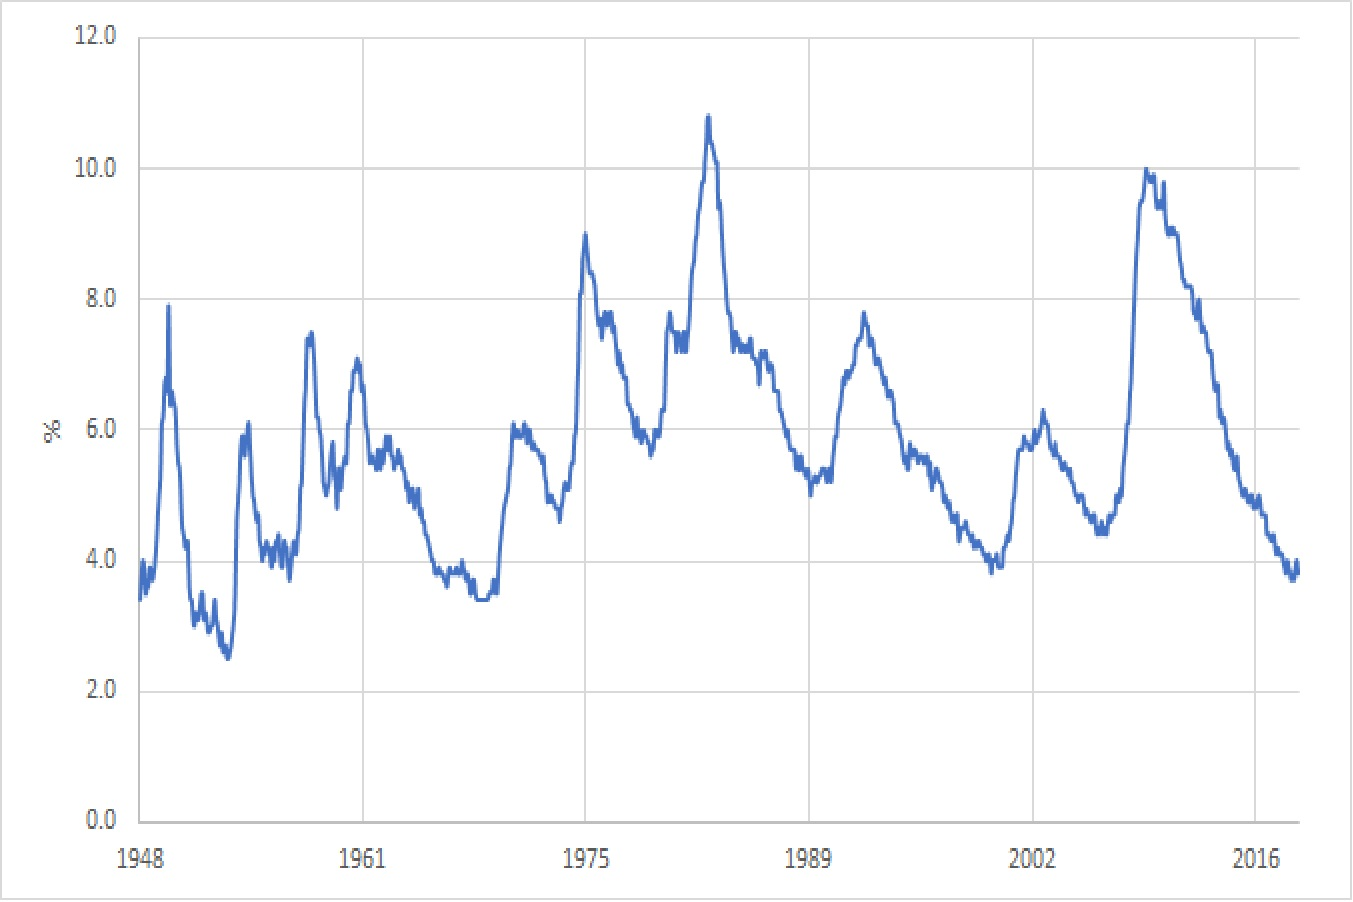
\includegraphics[width=0.50\textwidth]{unempl_US.jpg}
    \caption{Monthly unemployment rate for the population 16 years and over in the US. January 1948 to February 2019. Series LNS14000000 seasonally adjusted. Data from U.S. Bureau of Labor Statistics [BLS]: https://www.bls.gov/}
    \label{fig:unempl_US}
\end{figure}
% ----- END GRAPH

Finally, defining what money, is not an easy task since many economists have different opinions about this. For instance cash, bank accounts, savings accounts or credit cards all have a monetary value, yet there is no universal definition as to which ones account for the term \textit{money}. The lack of a common definition of money supply is a problem for the equation.

Additionally, the central bank does not control the money supply just by themselves. Creating and destroying money, as we know, can easily be made by the financial sector. By giving out more loans and creating money, M in the equation is directly influenced by the private sector.

Moreover, the central bank and commercial banks will have to work together. An increase in the money supply by the Central Bank requires the cooperation of the private sector first, especially if we think about the fact that targeting the interest rate is becoming a more common tool used by the central bank since banks will eventually enforce it. At the end of the day, private banks are in charge and not the central bank. The decisions made by the central bank will always depend on the rest of the economy and what they are willing to do.
\todo[inline]{These three paragraphs reflect that the criticism is done by taking the theory at face value, which is a weak critic. It can be improved.}

\subsection{The IS-LM Model}
\todo[inline]{The description of the IS-LM model need to be significantly improved.}
\label{sec:IS_LM}

\textbf{Money demand}. The quantity theory assumed a constant velocity, which made the money demand a linear function of nominal income. This model is instead based on Keynes' liquidity preference theory, where interest rates play a crucial role for money demand. Since a higher interest rate will increase the opportunity costs of holding money, which bears no interest, the demand for real money balances will be negatively related to the prevailing interest rate. But will be positively related to income, which increases the number of transactions for which money is needed.

\textbf{Money supply}. In this model the supply is assumed to be fixed by the Central Bank, which causes the supply curve to be vertical. An increase in the money supply shifts the curve to the right, whereas a decrease does the exact opposite.

As we can observe in figure \ref{fig:LM_curve}, the LM curve is constructed by plotting all the combinations of interest rate and income for which the money market is in equilibrium. As said, as real income increases, demand for real money balances grows, shifting the demand curve in the money market to the right. In the new money market equilibrium real money balances are unchanged, but the prevailing interest rate is now higher. Thus, there is a positive relationship between income and interest rate and the LM curve is upward sloping.

% ----- BEGIN GRAPH
\begin{figure}[h!]
  \centering
    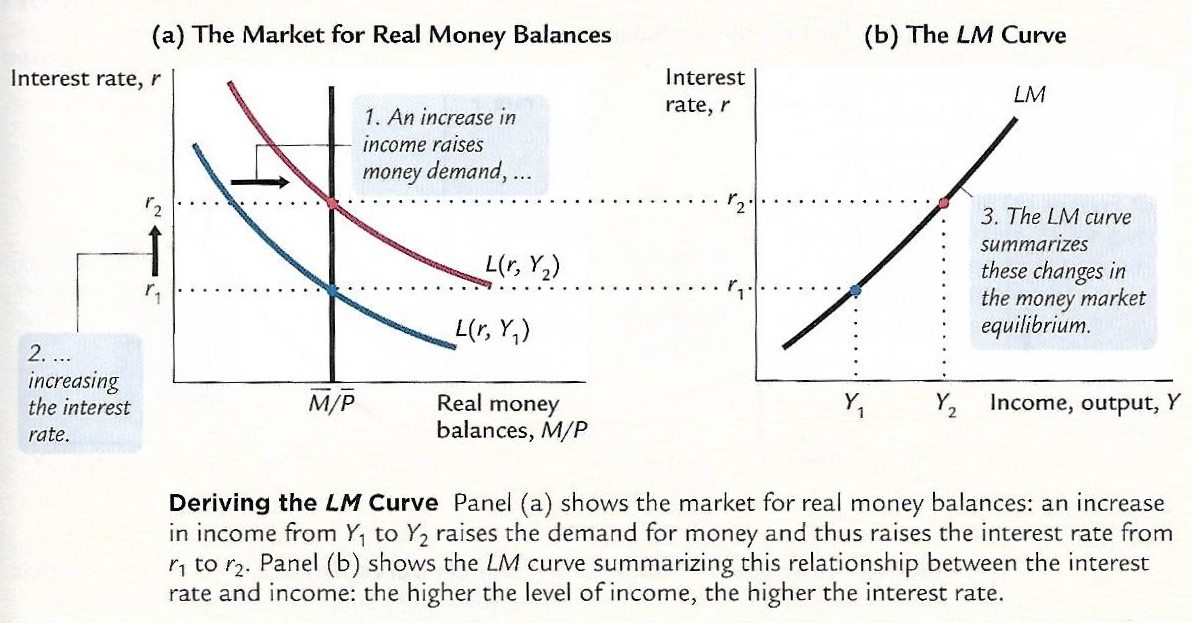
\includegraphics[width=0.65\textwidth]{LM_curve.jpg}
    \caption{Construction of the LM curve. Reprinted from: \citet*[p. 331]{Mankiw_2016}}
    \label{fig:LM_curve}
\end{figure}
% ----- END GRAPH

As figure \ref{fig:LM_curve_shift} shows, a reduction in the growth rate of the money supply will shift the money supply to the left, raising the interest rate for the same income level, which causes the LM curve to shift upwards.

% ----- BEGIN GRAPH
\begin{figure}[h!]
  \centering
    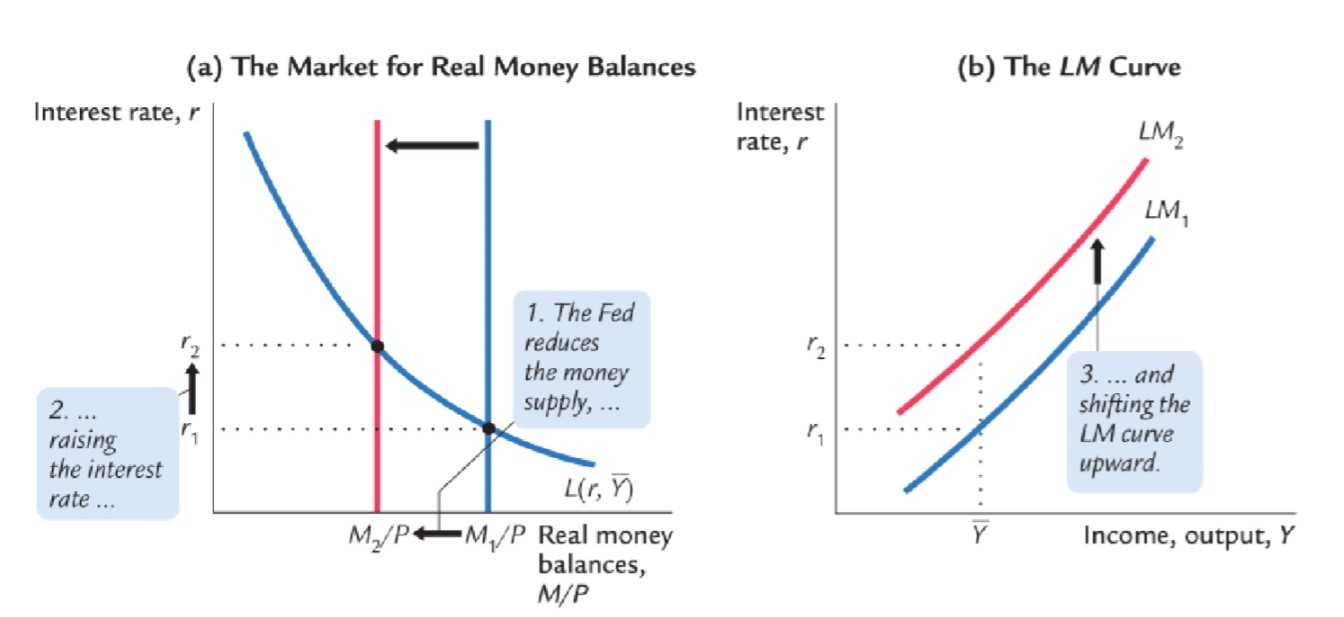
\includegraphics[width=0.75\textwidth]{LM_curve_shift.jpg}
    \caption{Decrease in the money supply and shift in the LM curve. Reprinted from: Lecture slides}
    \label{fig:LM_curve_shift}
\end{figure}
% ----- END GRAPH

The IS curve plots the combinations of interest rate and income for which the goods’ market is in equilibrium. The curve has to be downward sloping because a higher interest rate will lead to a lower equilibrium income, due to a reduction in planned investments.

By changing the price level and seeing how the equilibrium income varies in the IS-LM framework, we can construct the AD curve. An increase in the price level would decrease real money supply, raise the money market interest rate and shift the LM curve upwards, thus reducing equilibrium income at the intersection between IS and LM. The AD curve will then be downward sloping in the Y – P diagram.

The policy implications of the IS-LM model are very straightforward. When the economy is facing a recession, an expansionary monetary policy would reduce the interest rate, stimulating investments and increasing output. Eventually, as demand grows faster than the rate at which supply adjusts, inflation would arise, causing a reduction in the real money supply, which will reverse the initial stimulus.
\todo[inline]{The discussion of the policy implications needs more richness and to be deeper. There is much more in the IS-LM model than the superficial implications.}

When the economy is overheating, reducing the growth rate of money supply would increase the interest rates, which would decrease aggregate demand and slowdown inflation.

In the long-run, a higher growth rate of the money supply would not have an effect on the real variables but will only feed inflation. Average inflation over a certain period will then be equal to the average of the growth rate of money supply.

Under the IS-LM model the central bank should try to keep a growth rate of money supply that is consistent with its inflation target but could temporarily deviate from it to respond to shocks.
%--------------------------------------------------------------------------------------------------

% ---- The Basic Theory and the Data --------------------------------------------------------------
\section{The Basic Theory and the Data}
\label{sec:Basic_Theory_Data}
There is one policy implication that is equal for the Quantity Theory and the IS-LM framework, and it is that a permanently higher growth rate of money supply should lead to inflation in the long run.

It's important to clarify first how M is defined as money demand. As we have already seen in the section about the Quantity Theory of Money, M stands for the money stock. However, in reality there are different monetary aggregates that one could take into consideration. The Fed, for instance, reports two measures of money: M1 and M2. And unfortunately, the two do not tend to move necessarily together.
\begin{itemize}
  \item \textbf{M1} is the definition of money that contains the assets with the highest liquidity. It therefore represents the total sum of cash (notes and coins), travellers check and demand deposits.
  \item \textbf{M2} is a broader definition of money, that contains also less liquid assets. It includes, in addition to M1, savings deposits, small-denomination certificates of deposit and other money market asset on which checks can be written.
\end{itemize}

% ----- BEGIN GRAPH
\begin{figure}[h!]
  \centering
    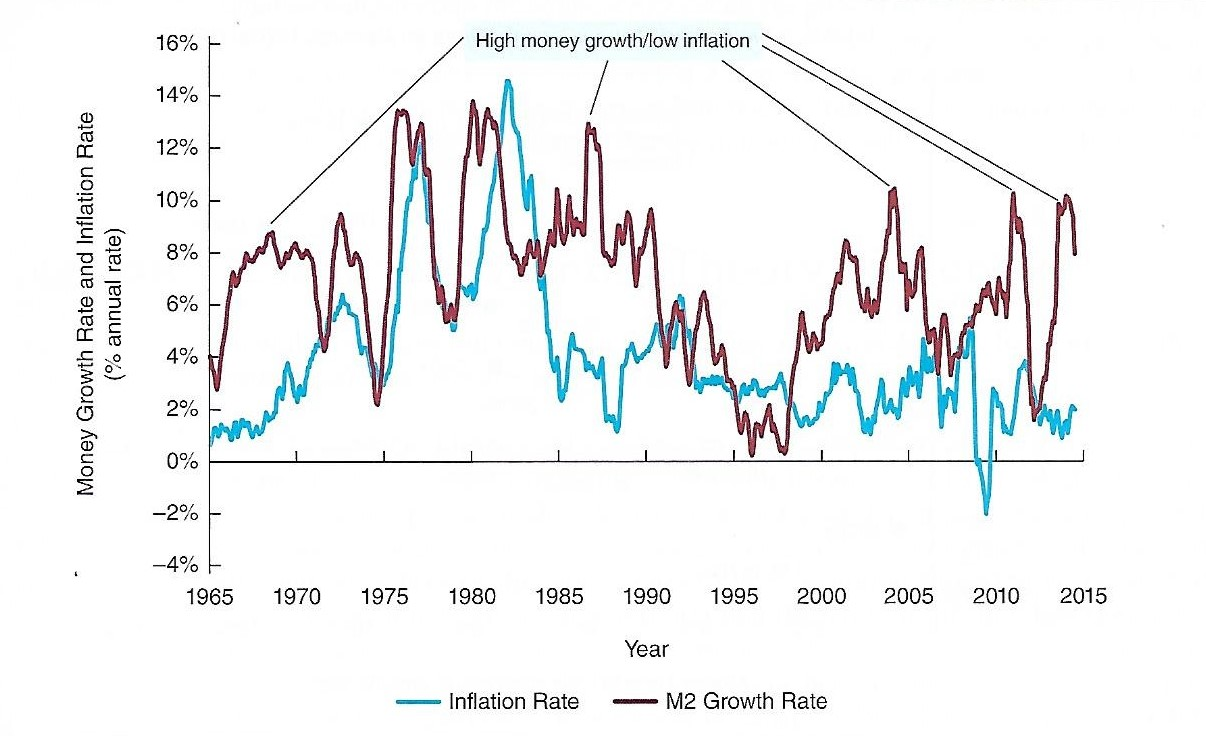
\includegraphics[width=0.60\textwidth]{SR_money_inflation.jpg}
    \caption{Annual inflation and annual money growth rate for the US. Period 1965-2013. Original data from Federal Reserve Bank of St. Louis, FRED database: http://research.stlouisfed.org/fred2/. Reprinted from: \citet*[p. 532]{Mishkin_2016}}
    \label{fig:SR_money_inflation}
\end{figure}
% ----- END GRAPH

First, we look at the relationship between money growth and inflation in the short run. Figure \ref{fig:SR_money_inflation}\todo{Get raw data and plot it using own format. Why seasonally adjust?} below shows the relationship between the annual growth rate of M2 and the annual inflation rate with a 2-year lag. If we define the long run as a decade, then we are looking at a short run relationship. Certainly, the relationship between the two variables does not seem as tight as postulated by the quantity theory and inflation in this case doesn't seem to be explained only by the growth rate of money supply. \citet*[p. 530]{Mishkin_2016} argues that the weak relationship signals a short run stickiness of prices and wages.

% ----- BEGIN GRAPH
\begin{figure}[h!]
  \centering
    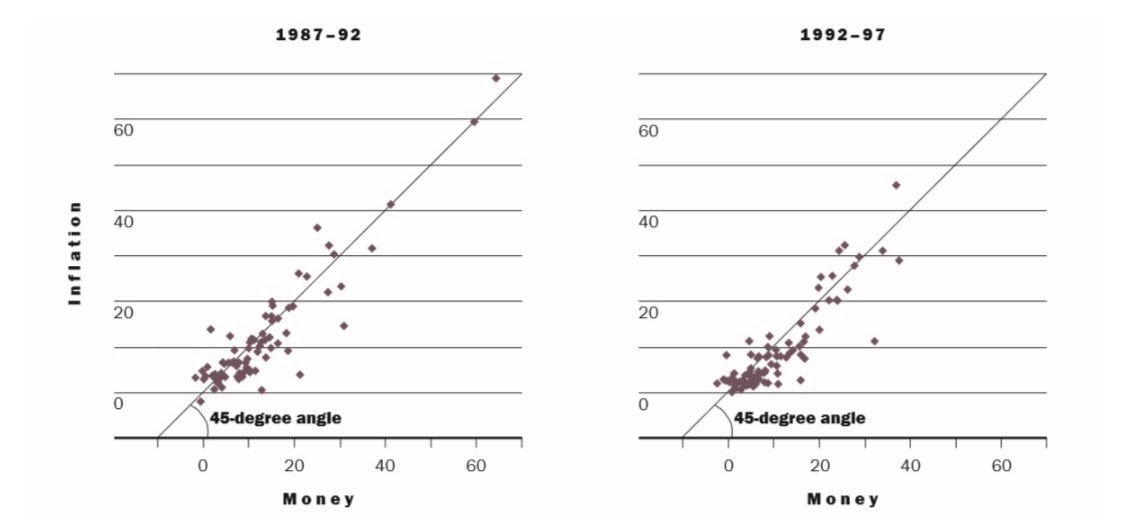
\includegraphics[width=0.70\textwidth]{Money_inflation_across_countries.jpg}
    \caption{Relationship between GDP deflator annualized and annualized growth rate of money across countries. 80 countries for 1987-1992 and 81 countries for 1992-1997. Original data from: International Monetary Fund (1999). \textit{International Financial Statistics}. Reprinted from: \citet*[p. 40]{Dwyer_Hafer_1999}}
    \label{fig:money_inflation_countries}
\end{figure}
% ----- END GRAPH

Figure \ref{fig:money_inflation_countries} depicts the 5-year average growth rate of money relative to real income against the 5-year average inflation for different countries \citet*{Dwyer_Hafer_1999}. We are thus looking at a relationship over a longer term than the 2 years of the example above. Probably, still, we can see it more as a medium run relationship between the two variables.

The relationship between money growth and inflation seems pretty convincing, with the points lying near the more or less along the 45-degrees straight line. However, \citet*{DeGrauwe_Polan_2005} studied the cross-country relationship between those two variables and argued that the relationship for the long run is very strong, but mainly due to countries with hyperinflation. The authors make the point that this relationship is virtually non-existent for countries with a lower inflation rate and might explain why the time series data for the single countries struggle to find a correlation.
\todo[inline]{There is much more to get from \citet*{DeGrauwe_Polan_2005} and the related literature.}

\subsubsection{Oil shocks}
\label{subsub:oil_shocks}
% ------------------
% Check references
%-----------------
\citet{Blanchard_Gali_2010} argue that there have been four large oil shocks in the years 1973, 1979, 1999, 2002. Those were episodes where global oil prices grew by more than 50\% and remained higher for at least one year. In Figure \ref{fig:oil} the inflation rate, as measured by the CPI, and the real oil prices are plotted. The relationship seems much closer than it was for money growth rate and inflation. Notice in particular that the two first oil shocks were also accompanied by huge surges in inflation for the US.
\todo[inline]{There is much juice to get from \citet{Blanchard_Gali_2010}}

% ----- BEGIN GRAPH
\begin{figure}[h!]
  \centering
    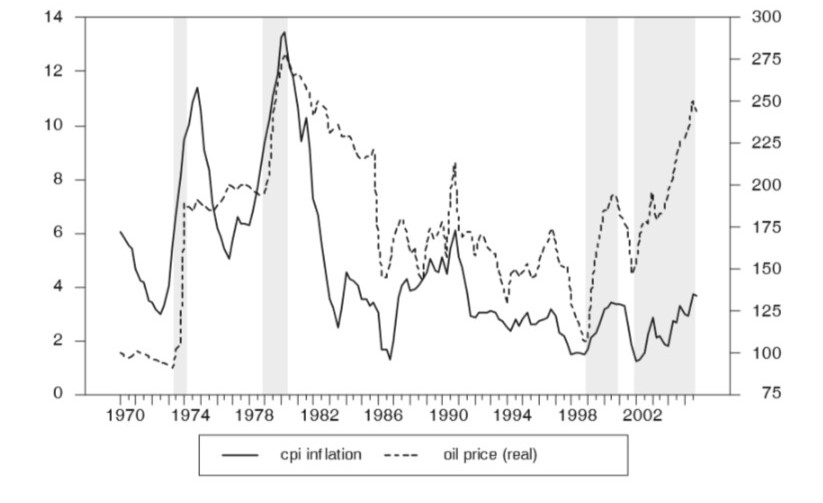
\includegraphics[width=0.75\textwidth]{Oil_shocks_inflation.jpg}
    \caption{Log of real oil price, normalized by GDP deflator, and annual CPI inflation in the US. 1950-2005. Reprinted from: \citet*[p. 12]{Blanchard_Gali_2010}}
    \label{fig:oil}
\end{figure}
% ----- END GRAPH

\citet*{Blanchard_Gali_2010} estimate that inflation was particularly sensitive to oil prices in the 1970s and found that if oil prices increased by 10\%, inflation rose by 1\% with a lag of two to three quarters. \todo[inline]{What is the point that \citet*{Blanchard_Gali_2010} make?}

However, inflation caused by higher oil prices would not necessarily be inconsistent with the predictions of the AD-AS model (which is based on the IS-LM model). Shocks in the oil prices are a classical example of supply shock, which, by shifting the AS curve to the left, should temporarily increase inflation.\todo[inline]{Here there is an important missed point with respect the policy lessons from the IS-LM model. What is the policy recommendation of the IS-LM model when there is an exogenous increase in prices (like an oil shock)?}

\subsubsection{Credit cards invention}
\label{subsub:credit_cards_invention}
\todo[inline]{It's a good idea to have a section that explains how credit cards might have changed the relationship between money supply growth and inflation. However, there needs to be a clear exposition of the arguments that have been put forward in the literature. \citet{Geanakoplos_Dubey_2010} is a good starting point to explore the literature but there are other works that tackle the issue at hand more directly.}

\subsubsection{More/other criticism}
\todo[inline]{More criticism on the IS-LM Model can be added to this chapter. Some references to start exploring the literature are \citet{Cooley_LeRoy_1981}, \citet{Driscoll_Ford_1980}, \citet{Humphrey_1974}, or \citet*{McLeay_etal_2014}.}
%--------------------------------------------------------------------------------------------------

% =================================================================================================

% ===== INFLATION TARGETING =======================================================================
\chapter{From Money Targeting to Inflation Targeting}

% ----- Historical context ------------------------------------------------------------------------
\section{Historical Context}
\label{sec:Historical_Context}
\todo[inline]{It's a good idea to introduce the topic by giving historical perspective/context. However, this introduction needs to be clear and cannot rely on concepts that have not been yet explained. Good references to start exploring the literature is \citet{Svensson_2010}, \citet{Bernanke_Mishkin_1997}, and \citet{Mishkin_2001}.}

There was mounting empirical evidence that the link between monetary supply and inflation was not as strong as previously believed. This led to central bankers beginning to target levels of inflation. With the introduction of the Reserve Bank Act of 1989, New Zealand established the policy framework today referred to as inflation targeting and were by the early 1990s the first country to introduce an explicit inflation target.

Inflation targeting consists of a public announcement of a numerical inflation target and a high degree of transparency to the public about the objectives of the policy as well as tightened accountability of the central banks for meeting the announced objectives.

Central banks moving from money growth targeting to inflation targeting replaced money supply as the intermediate target and introduced the inflation forecast as the new intermediate (and final) target. As a result, the central banks gain some freedom over how they react to different economic circumstances, since the variables considered in taking decisions about monetary policy are no longer restricted to monetary aggregates. Every factor influencing inflation can be reflected on, such as the money supply and the exchange rate, without having a dominant variable but by acknowledging the net effect of them all. \todo{The chain of thought in this paragraph can be much better explained using simpler sentences. Trying to sound complex has negative value.}

This new interaction of a long-term commitment to price stability and freedom in using different policy instruments is known as constrained discretion and is an essential trait for the central banks to react to events in the short run in order to also stabilize the real economy. Hence, inflation targeting needs to be viewed as a framework, and not as a rigid rule, within which this constrained discretion can be applied. \todo[inline]{Why is this important? Background context missing. It can be explained in an easier way.}
%--------------------------------------------------------------------------------------------------

% ----- Unemployment and Inflation ----------------------------------------------------------------
\section{Unemployment and Inflation}
\label{sec:Unemployment_Inflation}
\todo[inline]{An introduction to the Phillips curve is missing. Such introduction needs to answer the following questions. What is the Phillips curve? What idea does it represent? What are its limitations? When explaining the limitations the focus of the discussion has to be that an observed correlation has been taken as an structural relationship for many authors thinking/modelling the effect of monetary policy on the economy.

Because the idea of a Phillips curve is an ongoing discussion in the literature. This is how it should be presented. This discussion has produced both theoretical and empirical work. Make sure you correctly represent both.

There is a big literature discussing the idea of a Phillips curve, its empirical validation, etc. Good starting points for a literature review are \citet{King_Watson_1994}, \citet{Lucas_1976}, \citet{Kool_2000}. }
%--------------------------------------------------------------------------------------------------

% ----- Managing Inflation ------------------------------------------------------------------------
\section{Managing Inflation}
\label{sec:Managing_Inflation}
\todo[inline]{A thorough introduction to the idea of managing inflation is missing. This section should start describing, in a clear and straightforward way, how Central Banks manage inflation. Then, the idea of the Taylor rule should be introduced. Importantly, the role of the Taylor rule versus the actual inflation managing done by Central Banks needs to be highlighted and clarified.}

The Taylor rule is based on five assertions:
\begin{itemize}
  \item There is a natural equilibrium towards which the economy tends to in the long run.
  \item In the long run there is also no substitution between unemployment and inflation (as the Phillips curve is vertical in the long run).
  \item As prices are rigid in the short run, fluctuations around the growth equilibrium are possible.
  \item These fluctuations are determined by expectations towards future decisions made by the central banks, especially the expected interest rate and inflation influenced by central bank behaviour.
  \item Decisions of central banks can be understood as policy rules, which implies that the nominal interest rate is the tool the central banks use to regulate economic fluctuations.
\end{itemize}

The simplified Taylor rule equation is:\todo{What is the context that leads us to label this version as \textit{simplified}?}
\begin{equation}
  \label{eq:taylor}
  i_t=i^{\star}+a(\pi_t-\pi^{\star})-b(u_t-u_n)\text{,}
\end{equation}

where $i_t$ is the policy rate, $i^{\star}$ is the nominal interest rate, $r_n$ is  the real interest rate, $a$ and $b$ are weight factors, $\pi_t$ and $\pi^{\star}$ are the targeted and actual inflation rates respectively, and $u_t$ and $u_n$ are the actual and natural unemployment rates.

The Taylor rule is not a rulebook, but just a framework used to explain central banks’ behaviour. In recent years there has been a trend for central banks to significantly deviate from what the Taylor rule suggests. \todo{This ideas needs to be expanded, better put in context, and explained more clearly.}
%--------------------------------------------------------------------------------------------------

% =================================================================================================

% ===== TIME INCONSISTENCY, CREDIBILITY, AND INDEPENDENCE =========================================
\chapter{Time Inconsistency, Credibility, and Independence}
% ----- Time Inconsistency ------------------------------------------------------------------------
\section{Time Inconsistency}
\label{sec:Time_Inconsistency}
\todo[inline]{Time inconsistency is a concept that is present in many fields of Economics, from Game Theory to Macroeconomics. This section needs to start describing what the concept is and how is related to policy (in general) and monetary policy.

Then, to illustrate the idea of time inconsistency an example can be used. The example used in class regarding the Phillips curve is a valid choice. However there is no need to explain what the Phillips curve is as that has been done in the previous chapter.}
%--------------------------------------------------------------------------------------------------

% ----- Credibility -------------------------------------------------------------------------------
\section{Credibility}
\label{sec:Credibility}
\todo[inline]{This section needs to start by connecting the issue of Time Inconsistency with why it's valuable for a central bank to be credible in front of the public. The connection between these two concepts is key.

Then, the section has to offer a good summary of the different mechanisms that have been discussed in the literature on how to establish credibility.}
%--------------------------------------------------------------------------------------------------

% ----- Central Bank Independence -----------------------------------------------------------------
\section{Central Bank Independence}
\label{sec:Central_Bank_Independence}
\todo[inline]{This section needs to start by explaining what a central independent bank is and why it might be relevant. CB's independce is relevant for many reasons. Some of these reasons are related to credibility and time inconsistency. Hence, we can connect this section to the previous ones explaining how CB's independence may affect credibility and time inconsistency. However, these are not the only reasons (and maybe not even the most important) why we think CB's independence is relevant.

There is a literature trying to measure what is the effect of the independence of the central bank and it's monetary policy. Reviewing that literature might be a good idea if the following two conditions are satisfied. The theory framework in which we think about CB's independence is clearly explained and understood. Second, the limitations of this empirical literature are clearly understood and put forward.}
%--------------------------------------------------------------------------------------------------
% =================================================================================================

% ===== EFFECTS OF INFLATION ======================================================================
\chapter{The Effects of Inflation}
Inflation is nowadays commonly associated with the general rise of prices and wages. This means that a person will not be able to get the same amount of goods and services after an increase in inflation for the same amount of money. It is also important to distinguish between a price rise on a few items and a general price rise. A price rise on a few items is not regarded as an inflation, as it can depend on i.e. lower supply.\todo[inline]{Maybe it's a good idea to explain what is the dictionary definition of inflation and what it means for us in Economics.}

% ----- Measurement -------------------------------------------------------------------------------
\section{Measurement}
\label{sec:Measurement}
There are several ways of how inflation can be measured, but one of the most frequently used measurements of inflation (or deflation) is CPI, Consumer Price Index. CPI examines how a basket of pre-determined goods and services, such as food and clothes, changes in price accordingly to the weighted average. It is constructed as a chain index, meaning that price changes for a given period is expressed how it differs against the immediately preceding period.

Another commonly used measurement is PPI, Producer Price Index, which measures price development from the producer’s perspective rather than the viewpoint of the consumer. This index measures the average development of selling prices received by domestic producers for their output. PPI is calculated by dividing the current value of a basket of representative goods received by the seller by the prices in the chosen base year. For example, in the U.S, the Bureau of Labor Statistics set the PPI base to 100 in 1982.

\todo[inline]{It's a good idea to have a section on inflation measurement. The section, after a brief introduction, can assume that the reader is familiar with the concepts and basic measurements. A good way to extend this section would be to dive on the biases and issues that the current measures of inflation (the CPI an the PPI) face. Also, there could be a discussion on how \textit{representative} it is the basket of goods used when computing the CPI and whether there are distributional phenomena that are not captured by this weighted average.}

%--------------------------------------------------------------------------------------------------

% ----- The Effects of Inflation ------------------------------------------------------------------
\section{The Effects of Inflation}
\label{sec:Effects_of_Inflation}
\todo[inline]{It is essential for this chapter to have a section on the effects of inflation. This section needs to start explaining that there are many aspects of life/economic activity that can be affected by inflation with different magnitudes (it's not the same to have hyperinflation than a moderate level of inflation \textit{eroding} savings). After listing all the potential effects of inflation, those that have had bigger consequences in the data need to be discussed in more detail. Data and/or historical examples should be used throughout.}


%--------------------------------------------------------------------------------------------------



% =================================================================================================

% ===== UNCONVENTIONAL MONETARY POLICY ============================================================
\chapter{Unconventional Monetary Policy}

% ----- Introduction ------------------------------------------------------------------------------
\section{Introduction}
\label{sec:Intro_Unconventional}
\todo[inline]{This chapter needs to start with an introduction to we understand by unconventional monetary policy. After such introduction one can set the focus on Quantitative Easing. In that case, the concept of QE also needs to be introduced and explained. A good reference point in the literature is: \citet*{Joyce_etal_2012}.}

In order to appreciate the \textit{unconventionality} of QE, as well as the special circumstances of the Great Recession, one must first delve into the period which preceded it. Since the fight against high inflation in the 1970's and 1980's, the central banks of advanced economies seemed to have settled on a safe and reliable toolkit to conduct their monetary policy. What we now call conventional monetary policy is defined by a framework of inflation targeting, whereby the main policy instrument is the short-term (interbank) interest rate and the goal is low and stable inflation. This common understanding of orthodoxy led to the development of relatively simple and virtually self-completing mechanisms like the Taylor rule, which for the most part fulfilled the central banks' mandate of keeping inflation under control.

Naturally, conventional monetary policy remains policymakers' preferred course of action even after the events of the past decade, as the Federal Reserve's renewed focus on short-term interest rates and gradual winding down of the balance sheet as we have slowly returned to more or less normal times goes to show. However, two circumstances have generally been recognized as posing unsolvable jigsaws for monetary orthodoxy. They are the \todo{Unnecessary appreciation.} infamous zero-lower-bound problem as well as a financial paralysis so consequential, that financial markets become unable to function as they should.

Let us first focus on the former possibility. The zero-lower-bound problem is based upon the presumption that, once short-term nominal interest rates are near or at zero, the central bank has run "out of bullets" to influence aggregate demand. This is due to the fact that attempting to lower the nominal interest rate further could prove ineffective, simply because people can always just hold non-interest-bearing cash instead, effectively always offering a zero-interest alternative. Such a situation was in fact the one in which the United States found themselves following the Fed's decision to lower the Federal Funds Rate (representative of the short-term nominal interest rate) to nearly zero in December 2008.\footnote{See \citet{Blinder_2010}.}

The second limitation of conventional monetary policy is observable in a financial crisis such as the one at the heart of the Great Recession. As mentioned above, under normal circumstances, the central bank focuses its attention on the short-term nominal interbank interest rate (the Federal Funds Rate in the USA), that is, the rate at which commercial banks are able to borrow excess reserves from one another overnight. But this rate is in fact of minor importance to aggregate demand when compared to longer-term rates such as corporate bond yields or the interest rate on mortgages or car-loans.\todo{Explain why and provide empirical evidence.}\footnote{See \citet{Blinder_2010}.} Therefore, monetary policy has always heavily relied on the financial system in order for its policy decisions to translate to the real economy. In a financial panic however, the financial system seizes up and is incapable of fulfilling its role of capital allocation. This leads to a breakdown of the crucial "transition mechanism" and turns conventional monetary policy tools completely ineffectual.\todo{This is a valuable narrative but instead of presenting it as a fact it should be presented as one possible explanation among others.}
%--------------------------------------------------------------------------------------------------

% ----- Some theory behind QE ---------------------------------------------------------------------
\section{Some Theory Behind QE}
\label{sec:Some_Theory_Behind_QE}
\todo[inline]{This is an important section in which the theoretical effects of QE should be discussed. As of now the writing style does not reflect the nature of a theory. That is, one (of many) possible effects/explanations.}

On the one hand, QE would work just as a conventional tool. A large-scale asset purchase expands the Central Bank's balance sheet, with reserves increasing on the liabilities side. This in turn leads to an increase in the monetary base, and hopefully also in the money supply. As the money supply grows, the economy is stimulated (Mishkin, 2016, p.429). The same reasoning lies behind an open market operation by the Central Bank, a conventional monetary tool used in times of economic orthodoxy in order to manipulate the short-term federal funds rate. This however wasn't the only or even the main goal of QE. As mentioned in the previous section, the financial paralysis witnessed at the onset of QE1 in 2008, meant that the Fed's actions wouldn't necessarily translate into meaningful changes in the credit markets that truly matter to aggregate demand. Therefore, it was hoped that QE would be able to directly influence these longer-term rates. But how was this supposed to be done?

The interest rate spreads between riskless, short-term treasuries and other assets are usually due to a mix of three causes: term premiums, liquidity premiums and risk premiums. Term premiums (widely represented by and understood as the yield curve) may be because of the so-called expectations theory, a basic no-arbitrage condition according to which long-term rates must be equal to the average short-term rate over the same period. Alternatively, term premiums may simply be a representation of a "preferred habitat", whereby investors simply prefer short-term securities, possibly due to the psychological imminence of the pay-off. Risk premiums are the compensation demanded by investors in order to shoulder private debt rather than the alternative government debt. Government debt is considered riskless because the issuer can simply print money if it ever runs in to trouble regarding payment. Liquidity premiums exist since short-term and riskless securities are a lot easier to sell (liquid) than their more rigid alternatives, mostly due to the reasons cited just above. These views form the assumption that a perfect substitutability between assets, whether it be regarding duration or issuance (government or private), does not exist. This assumption is important in validating QE because, without it, there would be no reason for the specific targeting of longer-term assets. However, one must still answer the question of how QE actually targets these causes.

Firstly, the private sector, having sold its long-term assets to the Central Bank, is left with a maturity mismatch between its assets and liabilities. The willingness to rebalance its balance sheet therefore arises, and so, the demand for long-term assets rises. As the Central Bank has purchased large amounts of long-term assets, the available quantity of such assets on the market has been reduced. This generates a rise in the asset prices, associated with a decrease in the term premiums and therefore in the interest rates. Secondly, the willingness of the Fed to purchase what were often (mis-) characterized as toxic assets and to do so whilst shedding riskless, short-term treasuries was meant to restore investor confidence and reduce the risk spread. Finally, the increased demand by the Fed on the one side and by the private sector on the other would greatly improve the liquidity of these securities and unfreeze the markets.

The final impact on aggregate demand would be achieved through several channels. The lower interest rates would get the credit flow, for which theses securities exist, working again and spur firms' investment and house-buying once again, for instance. Furthermore, the unfreezing of these markets would hopefully re-establish the "classical" transmission mechanism discussed earlier. On the other hand, because interest rates and prices always move in opposite directions, the decrease in interest rates would lead to an appreciation of these assets and of alternatives such as stocks, seeing as an increase in the price of one substitute leads to an increase in demand of the other. This would help shore up the balance sheets and capitalization of financial institutions (and other firms) holding these securities, thus stopping the haemorrhage and improving credit flows once more. Additionally, this appreciation would increase the wealth of consumers who own these assets and encourage consumption and investment.
%--------------------------------------------------------------------------------------------------

% ----- Evidence on QE ----------------------------------------------------------------------------
\section{Evidence on QE}
\label{sec:Evidence_QE}
\todo[inline]{It is crucial to write a section on the empirical evidence on QE. It is a great challenge to write such a section. Not all evidence falls on the same category. Some evidence is descriptive, that is, there is no support for causal interpretation of the relationships presented. Some other evidence has a better case to be interpreted as causal. In this section, both need to be combined. However, it needs to be crystal clear which type of evidence is being presented. Even withn the \textit{category} of causal evidence, some studies might present a better case than others.}

The large-scale bond purchases increased the Fed's total assets from \$800 billion around September 2007 to over \$4 trillion at the end of 2014 as shown in Figure \ref{fig:QE_assets}:

% ----- BEGIN GRAPH
\begin{figure}[h!]
  \centering
    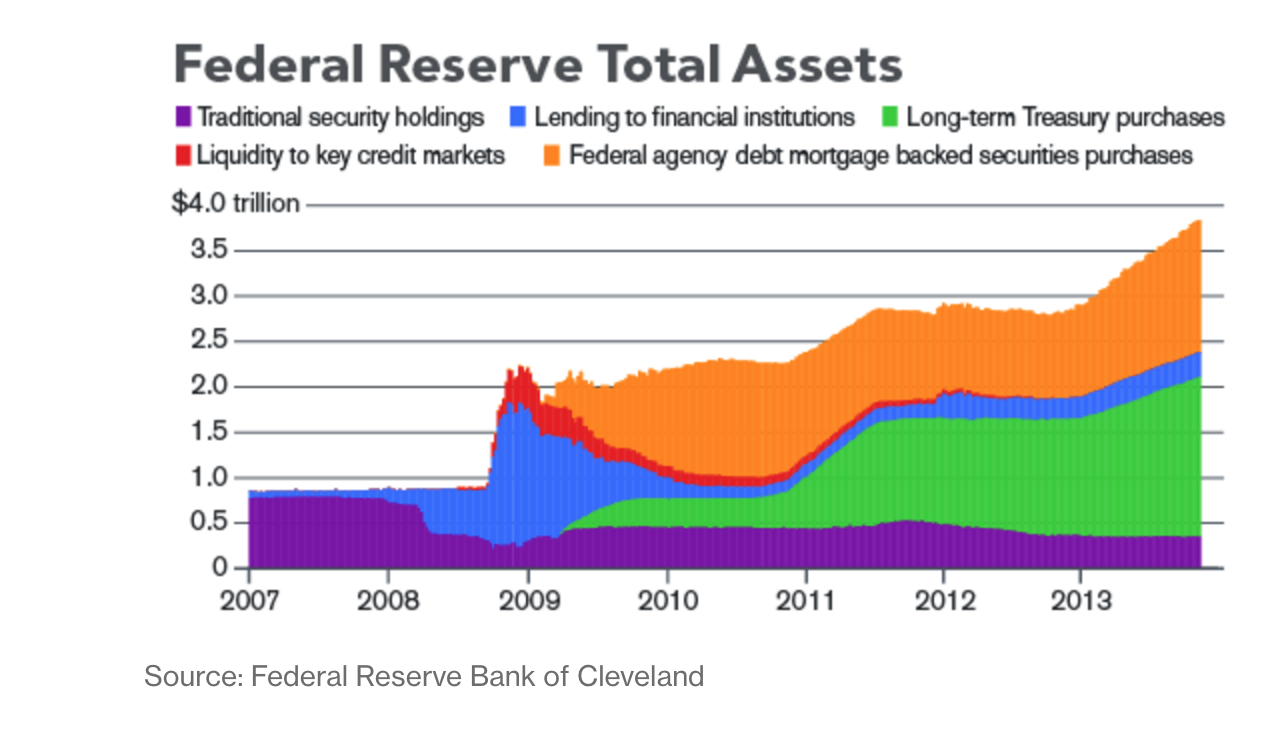
\includegraphics[width=0.75\textwidth]{QE_assets.png}
    \caption{Development of FED's assets.
    Source: Federal Reserve Bank of Cleveland.}
    \label{fig:QE_assets}
\end{figure}
% ----- END GRAPH
\todo[inline]{Source data for graph needs to be downloaded and graph needs to be created using own format. Better citation.}

In addition to this increase, the Fed altered the composition of its balance sheet by exchanging short-term securities for longer-term ones.  These transactions are visible by the increases of the violet and brown areas and the decrease of the green area in Figure \ref{fig:QE_assets}.

% ----- BEGIN GRAPH
\begin{figure}[h!]
  \centering
    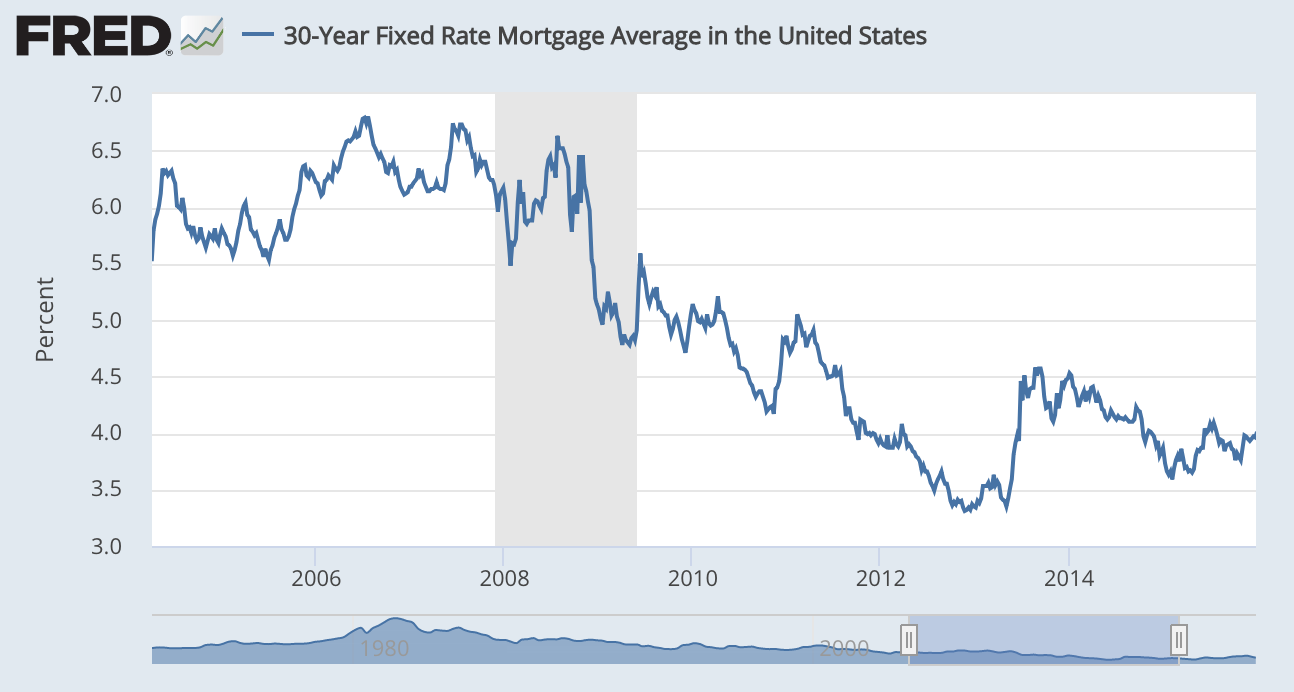
\includegraphics[width=0.75\textwidth]{QE_Mortgages.png}
    \caption{Development of 30-Year Mortgages interest rates. Federal Reserve Bank of St. Louis.}
    \label{fig:QE_Mortgages}
\end{figure}
% ----- END GRAPH
\todo[inline]{Source data for graph needs to be downloaded and graph needs to be created using own format. Better citation.}

One of the objectives was to save solvent banks by buying their toxic Mortgage-backed securities (MBS) in exchange for reserves, loans and treasuries. Another one was to prop up the MBS and other long-term markets and lower the residential mortgages interest rates to prevent an even bigger fall in the housing market and increase the aggregated demand.

% ----- BEGIN GRAPH
\begin{figure}[h!]
  \centering
    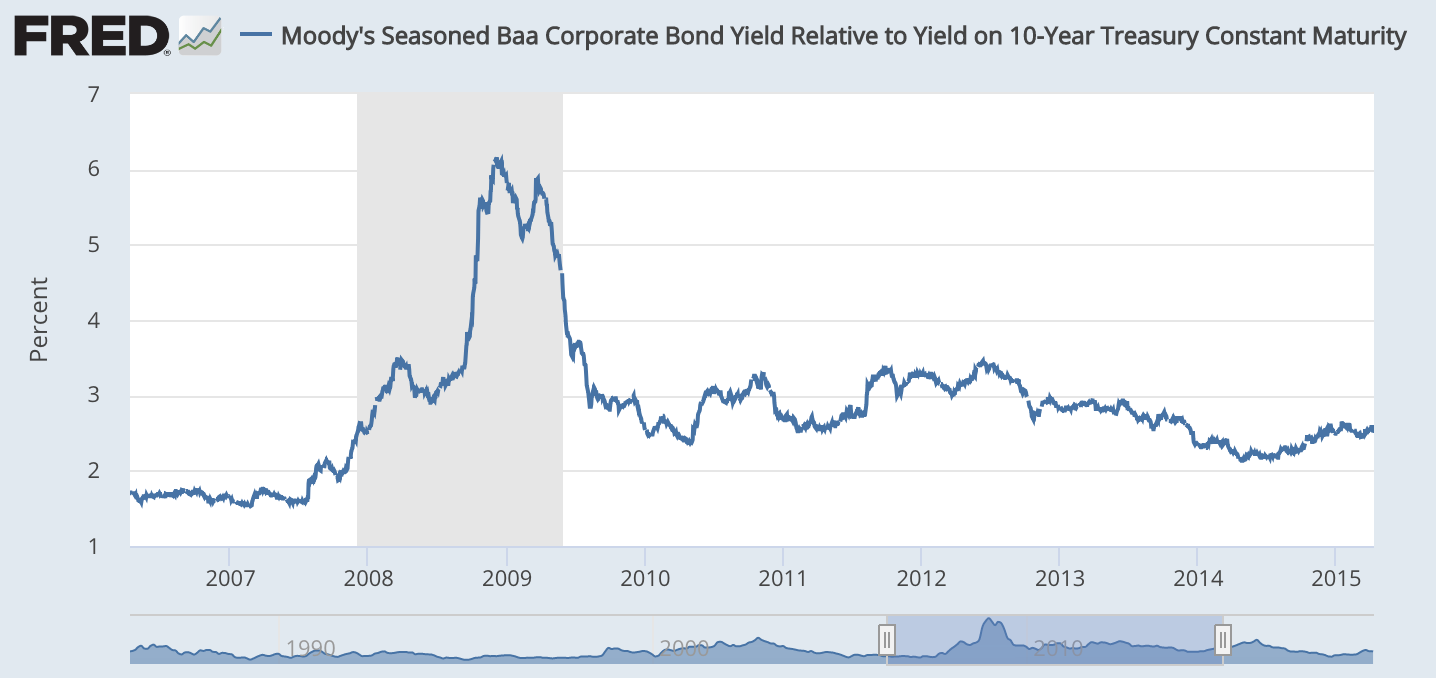
\includegraphics[width=0.75\textwidth]{QE_Baa.png}
    \caption{Development of risk spread between Moody's Baa Bonds and 10-Year Treasury Bonds. Federal Reserve Bank of St. Louis.}
    \label{fig:QE_Baa}
\end{figure}
% ----- END GRAPH
\todo[inline]{Source data for graph needs to be downloaded and graph needs to be created using own format. Better citation.}

As you see in Figure \ref{fig:QE_Mortgages} and \ref{fig:QE_Baa}, the interest rates of the long-term mortgages and the risk spread between 10-Year Treasury bonds and Moody's Baa Bonds (the lowest category of investment grade bonds) decreased over the period of the 3 QE's as intended by the Fed.

Another indicator that QE had a positive effect on the targeted markets is observable in Figure \ref{fig:QE_housing}. It seems that the three periods of QE stopped the large decline in housing prices. Furthermore, around the start of 2012, the prices started to increase again. This development implies, that the amount of mortgage lending went back up again which was intended by the Fed. One should still mention, that although the first two QE interventions stopped the fall in prices, the increase only happened shortly before the third intervention.

% ----- BEGIN GRAPH
\begin{figure}[h!]
  \centering
    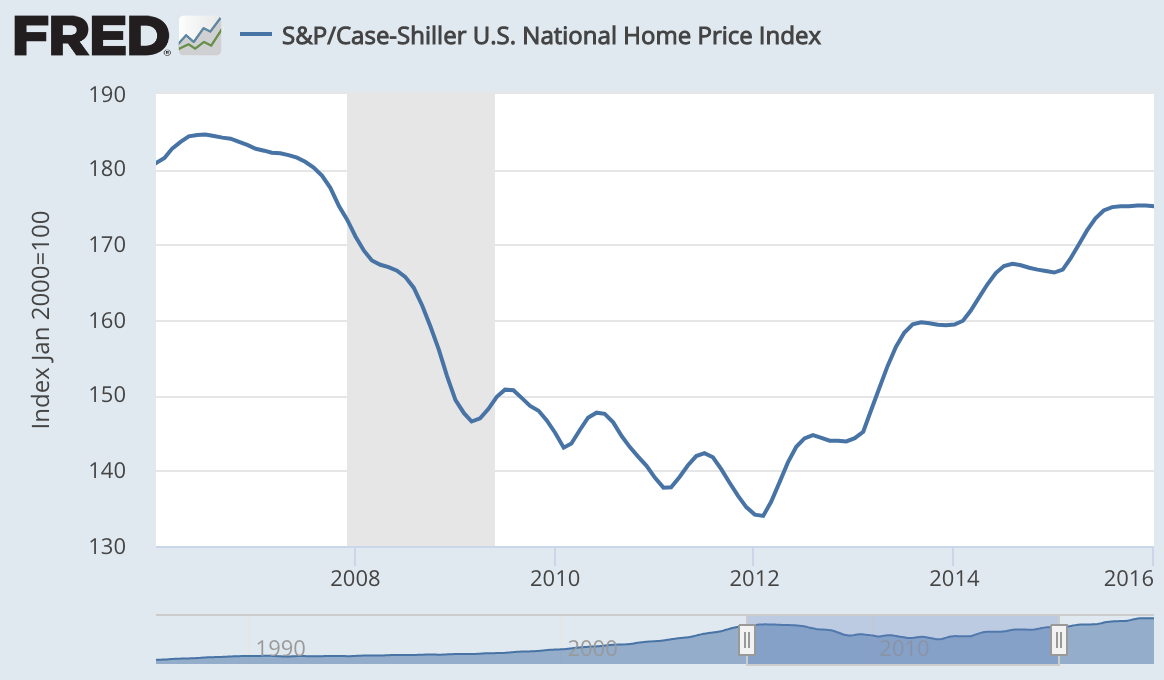
\includegraphics[width=0.75\textwidth]{QE_housing.png}
    \caption{Development of housing prices. Federal Reserve Bank of St. Louis.}
    \label{fig:QE_housing}
\end{figure}
% ----- END GRAPH
\todo[inline]{Source data for graph needs to be downloaded and graph needs to be created using own format. Better citation.}

\todo[inline]{Up to this point there is a reasonable good attempt to present descriptive evidence. What is missing is to point out that the evidence being presented is descriptive rather than causal. What is not necessary is to use a very well-defined narrative. Since the evidence is not causal, we cannot know for sure what is the exact chain of causal effects that generated the effects observed.}
%--------------------------------------------------------------------------------------------------

% =================================================================================================

% ===== FINANCIAL STABILITY =======================================================================
\chapter{Monetary Policy and Financial Stability}

% ----- Introduction ------------------------------------------------------------------------------
\section{Introduction}
\label{sec:Intro_Financial_Stability}
\todo[inline]{The introduction to this chapter is particularly important. This chapter needs to touch on many diverse topics. At the same time, some of these topics are not discussed in class. Hence, an effort to understand what is important concepts should be added to what is covered in class needs to be made.}


%--------------------------------------------------------------------------------------------------

% =================================================================================================

\part{Micro-founded Monetary Policy}
% ===== A CIA MODEL ===============================================================================
\chapter{A Cash-in-Advance Model}

% =================================================================================================

% ===== MONOPOLISTIC COMPETITION ==================================================================
\chapter{Monopolistic Competition}

% =================================================================================================

% ===== STICKY PRICES =============================================================================
\chapter{Sticky Prices}
\section{Introduction}
In the previous chapter, we introduced the notion of Monopolistic Competition and thus one key component of the New Keynesian Modell. This initial setting does not incorporate or seek to explain the effects of inflation. In fact, the optimisation problem, both retail and wholesale firms are faced with, in this initial approach only considers the current period and no past or future values. Since we wish to use this framework in order to explain inflation and its effects. Since money is only a unit of account in this model, we need to make price changes relevant to firms. Our goal for this chapter is therefore to provide some micro foundation for the interaction between the market and inflation by incorporating prices from different periods into the decision making of firms.

We achieve this by assuming, that it is costly for wholesale firms to change prices. Why may this assumption make sense? The classic example for sticky prices are menu costs. Say you run a restaurant and you wish to change the prices. Doing so implies that you have to print new menus, which is not free. So you may choose not to respond to all changes in demand or market prices. You would only respond if the increase in profits from a price change offsets the costs inherent in this price change. Beyond these relatively direct costs of price changes, consumers may also react to price changes. Say you change your menu prices quite significantly from one day to the next, your customers may be put off from visiting your restaurant by not knowing how much visiting your restaurant will cost them any given day. One would expect, that the more drastic your prices change, the greater this effect. The model we present in this section follows chapter 23 of \cite{chugh_2015}.
We assume that the real cost to wholesale firm $j$ for adjusting prices between periods is
\begin{equation}
	\frac{\Psi}{2}\bigg(\frac{P_t(j)}{P_{t-1}(j)}-1\bigg)^2
\end{equation}
with $ \Psi > 0 $. In effect this reflects what was outlined earlier. Costs are incured for both increasing and decreasing prices (When printing new menus, it is irrelevant wether or not prices increase or decrease). At the same time, the magnitude of price changes matters. The quadratic nature of this function implies that the costs are convex this gives rise to ``stickiness", as firms will prefer to adjust prices in small increments rather than all at once. $\Psi$ is some scalar factor, which essentially determines how relevant price adjustment costs are to our model. When $\Psi$ is zero we simply have the model from the previous chapter.

In our model, the perfectly competitive retail market implies that retail firms do not consider this additional cost. They still set price equal to marginal costs. This also means that demand from retail firms for the goods of wholesaler $j$ is unaffected and remains the same as in the previous chapter. I.e.
\begin{equation*}
	y(j)_t = \bigg(\frac{P_t}{P(j)_t}\bigg)^{\frac{\epsilon}{\epsilon-1}}y_t.
\end{equation*}

The next step is then to construct a new profit function for the Monopolistic wholesalers.
\section{Maximizing profits}
Nominal profits in any given period $t$ are given by
\begin{align*}
	P(j)_t\cdot y(j)_t -P_t \text{mc}_ty(j)_t-\underbrace{\frac{\Psi}{2}\bigg(\frac{P(j)_t}{P(j)_{t-1}}-1\bigg)^2\cdot P_{t}}_{\text{Nominal price adjustment costs}}
\end{align*}
Notice that this function contains $P(j)_{t-1}$. So the wholesalers choice of prices $P(j)_{t}$ in period $t$ also affects profits in the next period $t+1$. When maximising profits, a wholesaler in period $t$ must therefore consider discounted profits from the next period. This yields the following dynamic maximisation problem.

\begin{align}
	\begin{split}
	\max_{P(j)_t} \quad 
	& P(j)_t\cdot y(j)_t -P_t \text{mc}_ty(j)_t-\frac{\Psi}{2}\bigg(\frac{P(j)_t}{P(j)_{t-1}}-1\bigg)^2\cdot P_{t}+
	\\&\frac{\beta}{1+\pi_{t+1}}\bigg[P(j)_{t+1}\cdot y(j)_{t+1}-P_{t+1} \text{mc}_{t+1}y(j)_{t+1}-\frac{\Psi}{2}\bigg(\frac{P(j)_{t+1}}{P(j)_{t}}-1\bigg)^2\cdot P_{t+1}\bigg]
	\end{split}\\
	\text{where }\quad & y(j)_t = \bigg(\frac{P_t}{P(j)_t}\bigg)^{\frac{\epsilon}{\epsilon-1}}y_t
\end{align}
and $\frac{\beta }{ 1+\pi _{t+1} } $ is a nominal discount factor.

We will now seek to solve this maximization problem.
Solving the wholesalers maximization problem does not require a lagrangian. We do however need the derivative $\frac{\partial y}{\partial P(j)_t}$ as the wholesaler must consider the retailers response to a change in prices.
We denote by $y'(j)_t:=\frac{\partial y}{\partial P(j)_t}$ the derivative of demand for the products of firm $j$, $y(j)_t$, with respect to the price $P(j)$, set by this firm.  Since this is a key intermediate result for our maximization problem we begin here.
\begin{align}
	\frac{dy(j)_t}{dP(j)_t}&=\frac{d}{dP(j)_t}\bigg(\frac{P_t}{P(j)_t}\bigg)^{\frac{\epsilon}{\epsilon-1}}y_t\nonumber\\\nonumber
	&= \frac{\epsilon}{\epsilon-1}\bigg(\frac{P_t}{P(j)_t}\bigg)^{\frac{1}{\epsilon-1}}\frac{-P_t}{P(j)_t^2}y_t\\\nonumber
	&= \frac{-\epsilon}{\epsilon-1}\bigg(\frac{P_t}{P(j)_t}\bigg)^{\frac{1}{\epsilon-1}}\frac{P_t}{P(j)_t}\frac{1}{P(j)_t}y_t\\\nonumber
	&= \frac{\epsilon}{1-\epsilon}\underbrace{\bigg(\frac{P_t}{P(j)_t}\bigg)^{\frac{\epsilon}{\epsilon-1}}y_t}_{=y(j)_t}\frac{1}{P(j)_t}\label{eq: y'} \\
	&=\frac{\epsilon}{1-\epsilon}\frac{y(j)_t}{P(j)_t}
\end{align}
Another key function that we will take the derivative off, before proceeding with the maximization problem as a whole, is the price adjustment cost function. Let us first consider the cost function in period $t$.
\begin{equation}
	\frac{d}{dP(j)_t}\frac{\Psi}{2}\bigg(\frac{P_t(j)}{P_{t-1}(j)}-1\bigg)^2
\end{equation}
Finding this derivative requires us to use the chain rule: $\frac{d}{dx}f(u(x))=f'(u(x))u'(x)$. In the case of the cost function, 
\begin{align}
	\nonumber\frac{d}{dP(j)_t}\frac{\Psi}{2}\bigg(\frac{P(j)_t}{P_{t-1}(j)}-1\bigg)^2 &= \Psi\bigg(\frac{P_t(j)}{P_{t-1}(j)}-1\bigg)\frac{d}{dP(j)_t}\bigg(\frac{P_t(j)}{P_{t-1}(j)}-1\bigg)\\
	&=\Psi\bigg(\frac{P_t(j)}{P_{t-1}(j)}-1\bigg)\bigg(\frac{1}{P(j)_{t-1}}\bigg).\label{eq: adjust_t}
\end{align}
Although it appears to be quite similar, we will consider the cost function for period $t+1$ separately. We use the chain rule again, yielding
\begin{align}
	\nonumber\frac{d}{dP(j)_t}\frac{\Psi}{2}\bigg(\frac{P(j)_{t+1}}{P(j)_{t}}-1\bigg)^2 &= \Psi\bigg(\frac{P(j)_{t+1}}{P(j)_{t}}-1\bigg)\frac{d}{dP(j)_t}\bigg(\frac{P(j)_{t+1}}{P(j)_{t}}-1\bigg)\\
	&=\Psi\bigg(\frac{P(j)_{t+1}}{P(j)_{t}}-1\bigg)\bigg(\frac{-P(j)_{t+1}}{P(j)_{t}^2}\bigg)\nonumber\\
	&=-\Psi\bigg(\frac{P(j)_{t+1}}{P(j)_{t}}-1\bigg)\frac{P(j)_{t+1}}{P(j)_{t}^2}\label{eq: adjust_t1}
\end{align}

Having determined how price adjustment costs and demand respond to changes in wholesaler prices, we are now ready to proceed with the Wholesale Firms maximization problem as a whole. We begin by taking the derivative of the wholesalers profit function with respect to $P(j)_t$.
 \begin{align}\nonumber
	&\,\frac{d}{dP(j)_t}\bigg(P(j)_t\cdot y(j)_t -P_t \text{mc}_ty(j)_t-\frac{\Psi}{2}\bigg(\frac{P(j)_t}{P(j)_{t-1}}-1\bigg)^2\cdot P_{t}
	\\&\quad\nonumber+\frac{\beta}{1+\pi_{t+1}}\bigg[P(j)_{t+1}\cdot y(j)_{t+1}-P_{t+1} \text{mc}_{t+1}y(j)_{t+1}-\frac{\Psi}{2}\bigg(\frac{P(j)_{t+1}}{P(j)_{t}}-1\bigg)^2\cdot P_{t+1}\bigg]\bigg)\\\nonumber
	&=\underbrace{\frac{d}{dP(j)_t}(P(j)_t\cdot y(j)_t)}_{\text{product rule}} - \frac{d}{dP(j)_t}P_t \text{mc}_ty(j)_t-\underbrace{\frac{d}{dP(j)_t}\frac{\Psi}{2}\bigg(\frac{P(j)_t}{P(j)_{t-1}}-1\bigg)^2}_\text{\eqref{eq: adjust_t}}\cdot P_{t}
	\\&\quad\nonumber-\frac{\beta}{1+\pi_{t+1}}\bigg[\underbrace{\frac{d}{dP(j)_t}\frac{\Psi}{2}\bigg(\frac{P(j)_{t+1}}{P(j)_{t}}-1\bigg)^2}_{\text{\eqref{eq: adjust_t1}}}\cdot P_{t+1}\bigg]\bigg)\\
	\begin{split}
		&=P(j)_t\cdot y'(j)_t + y(j)_t -P_t \text{mc}_ty'(j)_t-\Psi\cdot\bigg(\frac{P(j)_t}{P(j)_{t-1}}-1\bigg)\frac{P_{t}}{P(j)_{t-1}}\\ &\quad+\frac{\beta}{1+\pi_{t+1}}\bigg[\Psi\cdot\bigg(\frac{P(j)_{t+1}}{P(j)_{t}}-1\bigg)\cdot \frac{P(j)_{t+1}}{P(j)_t^2}\cdot P_{t+1}\bigg]
	\end{split}
\end{align}
By substituting \eqref{eq: y'} for $y'(j)_t$, we find
\begin{align}
	&=\frac{\epsilon}{1-\epsilon}y(j)_t + y(j)_t - \frac{\epsilon}{1-\epsilon}\frac{P_t}{P(j)_t}y(j)_t\text{mc}_t \nonumber\\
	&\quad+\Psi\bigg[\frac{\beta}{1+\pi_{t+1}}\bigg(\frac{P(j)_{t+1}}{P(j)_{t}}-1\bigg)\frac{P_{t+1}}{P(j)_t}\frac{P(j)_{t+1}}{P(j)_t} -\bigg(\frac{P(j)_t}{P(j)_{t-1}}-1\bigg)\frac{P_{t}}{P(j)_{t-1}}\bigg]\nonumber\\
	&=\bigg(\frac{\epsilon}{1-\epsilon}+1\bigg)\bigg(\frac{P_t}{P(j)_t}\bigg)^{\frac{\epsilon}{\epsilon-1}}y_t - \frac{\epsilon}{1-\epsilon}\bigg(\frac{P_t}{P(j)_t}\bigg)\bigg(\frac{P_t}{P(j)_t}\bigg)^{\frac{\epsilon}{\epsilon-1}}y_t\text{mc}_t \\&\quad+\Psi\bigg[\frac{\beta}{1+\pi_{t+1}}\bigg(\frac{P(j)_{t+1}}{P(j)_{t}}-1\bigg)\frac{P_{t+1}}{P(j)_t}\frac{P(j)_{t+1}}{P(j)_t} -\bigg(\frac{P(j)_t}{P(j)_{t-1}}-1\bigg)\frac{P_{t}}{P(j)_{t-1}}\bigg]\nonumber\\
	\begin{split}
	&=\frac{1}{1-\epsilon}\bigg(\frac{P_t}{P(j)_t}\bigg)^{\frac{\epsilon}{\epsilon-1}}y_t - \frac{\epsilon}{1-\epsilon}\bigg(\frac{P_t}{P(j)_t}\bigg)^{\frac{2\epsilon-1}{\epsilon-1}}y_t\text{mc}_t \\&\quad+\Psi\bigg[\frac{\beta}{1+\pi_{t+1}}\bigg(\frac{P(j)_{t+1}}{P(j)_{t}}-1\bigg)\frac{P_{t+1}}{P(j)_t}\frac{P(j)_{t+1}}{P(j)_t} -\bigg(\frac{P(j)_t}{P(j)_{t-1}}-1\bigg)\frac{P_{t}}{P(j)_{t-1}}\bigg]\nonumber
	\end{split}
	\end{align}
	This yields the First order condition for prices set by wholesale producers in order to maximise profits.
	\begin{equation}
	\begin{split}
		\frac{1}{1-\epsilon}\bigg(\frac{P_t}{P(j)_t}\bigg)^{\frac{\epsilon}{\epsilon-1}}y_t - \frac{\epsilon}{1-\epsilon}\bigg(\frac{P_t}{P(j)_t}\bigg)^{\frac{2\epsilon-1}{\epsilon-1}}y_t\text{mc}_t &\\+\Psi\bigg[\frac{\beta}{1+\pi_{t+1}}\bigg(\frac{P(j)_{t+1}}{P(j)_{t}}-1\bigg)\frac{P_{t+1}}{P(j)_t}\frac{P(j)_{t+1}}{P(j)_t}&\\- \bigg(\frac{P(j)_t}{P(j)_{t-1}}-1\bigg)\frac{P_{t}}{P(j)_{t-1}}\bigg]&=0\label{eq:FOC}
	\end{split}
	\end{equation}
This condition, is a little nondescript and not particularly suitable for further analysis. Notice however, that $\Psi = 0$ would yield the first order condition from the previous chapter. I.e. without price adjustment costs. When $\Psi\geq 0$ however, next period inflation, past current and future prices of the wholesale firm $j$ and prices set by retailers must align for an equilibrium. 
\section{Symmetric Equilibrium and the New Keynesian Phillips curve}
In order to gain a little more insight into what the first order condition \eqref{eq:FOC} means, we restrict our analysis to a symmetric equilibrium. In a symmetric equilibrium $P_t = P(j)_t\quad \forall j \in (0,1).$ This follows from all wholesalers having the same market power and the same costs in our model. The prices $P(j)_t$ should be identical for all $j$ and it is optimal for a retail firm to purchase equal amounts from all wholesalers. The fact that the retail market has perfect competition then implies that profits of the retailer are $0$ and as such $P_t = P(j)_t$. When just considering this equilibrium, we can therefore drop all $j$'s from our first order condition, yielding
\begin{align}
	\begin{split}
	\frac{1}{1-\epsilon}(1)^{\frac{\epsilon}{\epsilon-1}}y_t - \frac{\epsilon}{1-\epsilon}(1)^{\frac{2\epsilon-1}{\epsilon-1}}y_t\text{mc}_t +\Psi\bigg[\frac{\beta}{1+\pi_{t+1}}\bigg(\frac{P_{t+1}}{P_{t}}-1\bigg)\bigg(\frac{P_{t+1}}{P_t}\bigg)^2&\\- \bigg(\frac{P_t}{P_{t-1}}-1\bigg)\frac{P_{t}}{P_{t-1}}\bigg]&=0.
	\end{split}\label{eq:symstep1}
\end{align}
Since the inflation rate is defined as $\pi_t := \frac{P_{t}-P{t-1}}{P_{t-1}}=\frac{P_t}{P_{t-1}}-1$ we can rewrite equation \eqref{eq:symstep1} as 
\begin{align}
	\Psi\bigg[\frac{\beta}{1+\pi_{t+1}}\pi_{t+1}\bigg(\underbrace{\frac{P_{t+1}}{P_t}}_{1+\pi_{t+1}}\bigg)^2- \pi_t\underbrace{\frac{P_t}{P_{t-1}}}_{1+\pi_t}\bigg]&=\frac{-y_t}{1-\epsilon}+\frac{\epsilon}{1-\epsilon}y_t\text{mc}_t\\
	-\Psi\pi _t(1+\pi_t)&=-\frac{y_t}{1-\epsilon}(1-\epsilon\cdot\text{mc}_t)-\Psi\bigg(\frac{\beta\pi _{t+1}}{1+\pi_{t+1}}\bigg)(1+\pi _{t+1})^2\nonumber\\
	\pi _t(1+\pi_t)&=\frac{y_t}{(1-\epsilon)\Psi}(1-\epsilon\cdot\text{mc}_t)+\beta\pi_{t+1}(1+\pi _{t+1})\label{eq:nkPhilips}
\end{align}
Equation \eqref{eq:nkPhilips} relates output under Monopolistic competition with sticky prices to the present and future interest rate. It is known as the New Keynesian Philips Curve.
\begin{equation*}
	\pi _t(1+\pi_t)=\frac{y_t}{(1-\epsilon)\Psi}(1-\epsilon\cdot\text{mc}_t)+\beta\pi_{t+1}(1+\pi _{t+1})
\end{equation*}
This Phillips curve implies that inflation is dependent on the marginal costs of production. All else being equal, an increase in marginal costs implies an increase in inflation.
To illustrate this, we take the derivative off this philips curve with respect to marginal costs.
\begin{align*}
	\frac{\partial\pi _t(1+\pi_t)}{\partial \text{mc}_t} &= -\frac{\epsilon y_t}{(1-\epsilon)\Psi}\\
	&= \frac{\epsilon y_t}{(\epsilon-1)\Psi}
\end{align*}
Since $\epsilon>1,\,\Psi>0,\,y_t>0$ this first order derivative is greater than $0$. Inflation is therefore increasing in marginal costs. This implies, that an increase in wages for example would increase inflation. If higher unemployment leads to lower wages, implying lower marginal costs and thus lower inflation, then we have a similar relationship between unemployment and inflation as in the standard Phillips curve. 

One key difference is the inclusion of next period inflation in the New Keynesian Phillips Curve. This means that present inflation is dependent on next periods inflation. This is a dynamic relationship that is not present in the classic model and reflects the importance of next period prices for the wholesalers profit maximization problem.
\section{Our Model and Sticky Prices in general}
The basis for the New Keynesian Philips Curve and sticky prices that we have used here are quadratic price adjustment costs to wholesalers. This is a concept initially proposed by \cite{Rotemberg}. There is however a much broader selection of proposed causes for sticky prices.  \cite{CALVO1983383} for example assume that individual firms are only able to alter their prices in random intervals, independent of one another. The resulting New Keynesian Philips Curve is quite similar however.  Wether or not prices are actually sticky, if so which products and how to explain this stickiness appears to be unresolved. There is some evidence that runs counter to Rotembergs quadratic cost function. In particular, it does not appear that prices are updated as regularly, as a convex cost function would suggest \cite{KLENOW2010231}. Nevertheless, this approach provides an easily understood approach to include price stickiness and derive a New Keynesian Philips Curve.
% =================================================================================================

% ===== OPTIMAL POLICY WITH STICKY PRICES =========================================================
\chapter{Optimal Policy with Sticky Prices}

% =================================================================================================

% ...

% \appendix
% \chapter{First Appendix}

\backmatter
\bibliography{monetary.bib}


\end{document}
